\documentclass[11pt]{book} % 11pt font
\usepackage{amsmath}
\usepackage{amsfonts}
\usepackage{bm}
\usepackage{graphicx}
\usepackage{mathtools}
\usepackage{physics}
\usepackage{pgfplots}
\usepackage{accents}
\usepackage{geometry}
\usepackage{caption}

% my custom commands
% ------------------
% note command
\newcommand{\note}[1]{\textsf{\textcolor{red}{#1}}}
% multi-line comment command
\newcommand{\comment}[1]{}
\newcommand{\del}{\bm{\nabla}}
\newcommand{\partder}[2]{\frac{\partial #1}{\partial #2}}
\graphicspath{{./images}}


% -------------------------
% BEGINNING OF THE DOCUMENT
% -------------------------
\begin{document}

\chapter{Ben Farr, Winter 2025}
\section{Newtonian gravity}
The newtonian formula for gravitational attraction is $F = \frac{Gm_1 m_2}{r_{12}^2}$. This formula unfortunately doesn't agree with special relativity, in that the attractive force has no speed of light propogation.
Although the shift to general relativity will change this a bit, a few things still persist. Gravity is not screened by opposing charges, and it is extremely long range in both the newtonian and einsteinian description.

Comparing the relative forces between different fundamental forces we can take a pair of protons as our example:
\begin{align*}
	\frac{F_\text{grav}}{F_{EM}} &= \frac{Gm_p^2}{\frac{e^2}{4\pi\epsilon_0}} \\
	\frac{F_\text{grav}}{F_{EM}} &~ 10^{-36}
\end{align*}
This of course doesn't drive the motion of the universe as most charges end up screened on large scales.

Looking instead at the importance of using the generally relativistic formulation instead of the newtonian description we have another quantity we want to consider. The quantity $\frac{GM}{Rc^2}$ will describe the relative importance for gerneral relativity.
If we look at earth, we see a value of $10^{-9}$, which is only important for extremely precise measurements. For the sun we see $10^{-6}$, which ended up primarily showing up in the perihilion precession of mercury.
For Neutron stars we see a value of $0.1$. And finally looking at black holes we see at the event horizon $0.5$. Due to coincidence (potentially) it turns out we can calculate the excape velocity using newtonian mechanics.

\begin{figure*}[h]
	\centering
	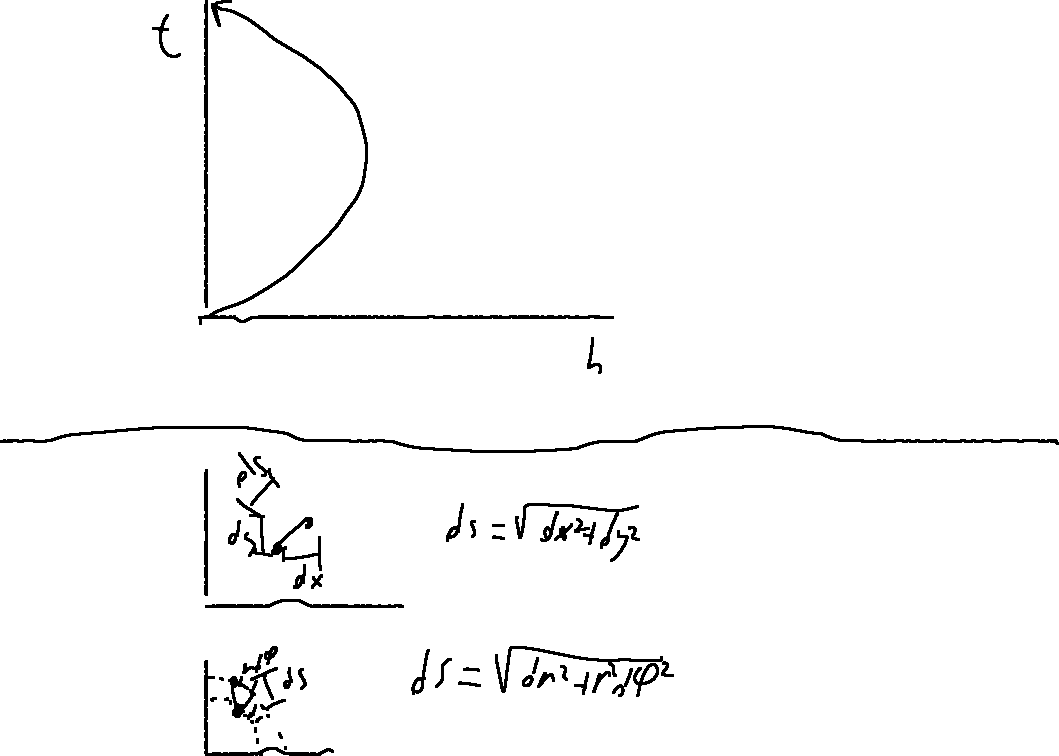
\includegraphics[width=10cm]{1-07-1.png}
	\caption*{Euclidean Geometries}
\end{figure*}
If we now seek to calculate the circumference of a circle using these two different coordinate systems:
\begin{align*}
	C &= \int ds \\
	C &= \int \sqrt{dx^2 + dy^2} \\
	C &= 2\int_-R^R \sqrt{1 + y'\ ^2}dx \\
	C &= 2R\int_-1^1 \frac{dv}{\sqrt{1-v^2}} \\
	C &= 2\pi R
\end{align*}
In the case of polar coordinates though:
\begin{align*}
	C &= \int ds \\
	C &= \int_0^{2\pi} R d\phi \\
	C &= 2\pi R
\end{align*}

We can see that both of these describe Euclidean geometries, but if we move to the Geometry on the surface of a sphere:

The line element is:
\begin{align*}
	ds^2 &= a^2 d\theta^2 + a^2\sin^2\theta d\phi^2
\end{align*}
We can w.l.o.g rotate our sphere such that our circle is moving along a curve where $\theta$ is constant. Therefore we have:
\begin{align*}
	ds &= a\sin\theta d\phi \\
	C &= a2\pi \sin\theta
\end{align*}
If instead we have a circle of radius r, on a sphere of radius a, we choose coordinates with varying $\theta$ but constant $\phi$, so:
\begin{align*}
	ds &= ad\theta \\
	r &= \int ds \\
	r &= \int _0^\theta ad\theta \\
	r &= a\theta \\
	C &= 2\pi a \sin \frac{r}{a}
\end{align*}
Which matches Euclidean geometry in the small r limit.

In GR we will often take a line element and try to use it to understand the underlying geometry. For example we consider $ds^2 = a^2(d\theta^2 f^2(\theta) d\phi^2)$. If we choose $\theta = \sin\theta$ then we are working on the surface of a sphere.
The first property we can not is that the line element is unchanged with $\phi$, so this must have a symetry around the z axis. If we look at $f(\theta) = \sin\theta(1-\frac{3}{4}\sin^2\theta)$, we end up with a peanut geometry.
\begin{figure*}[h]
	\centering
	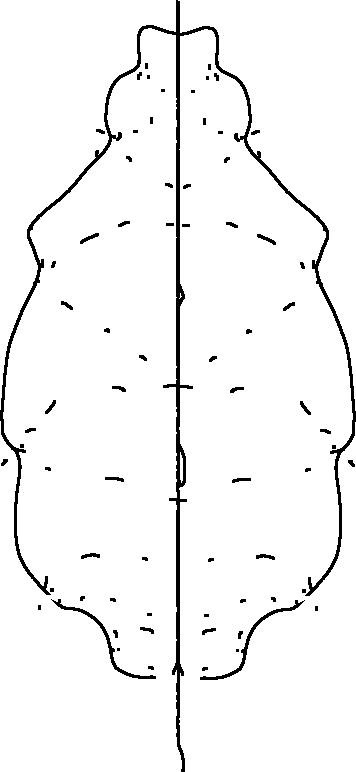
\includegraphics[width=10cm]{1-07-2.png}
	\caption*{Our general $f(\theta)$ geometry}
\end{figure*}

In an inertial frame an observer will have a set of coordinates $t$ such that $\frac{d^2x_i}{dt^2}=0$. A pair of inertial frames can differ by constant displacements, uniform velocities, and constant rotations.

Looking at a pair of frames that only differ by displacements $(x,y,z)$, $(x',y',z')$, if we have this displacement be $d$ along the x axis we know:
\begin{align*}
	x' &= x-d & y'&= y & z' &= z
\end{align*}
Instead for a rotation $\theta$ about the z axis:
\begin{align*}
	x' &= \sin\theta y + \cos\theta x &
	y' &= \cos\theta y - \sin \theta x &
	z' &= z
\end{align*}
If we inestead have a uniform velocity about the x axis, we instead have:
\begin{align*}
	x' &= x -vt' &
	y' &= y &
	z' &= z
\end{align*}

For a point mass experience a gravitational attraction we see:
\begin{align*}
	\bm{F} &= -\frac{GmM}{r^2} \hat{e}_r \\
	\Phi(\bm{x}) &= -\frac{GM}{r} \\
	\Phi(\bm{x}) &= -\frac{GM}{|\bm{x} - \bm{x}_A|}
\end{align*}
If we add multiple point masses:
\begin{align*}
	\Phi(\bm{x}) &= \sum_A-\frac{GM_A}{|\bm{x} - \bm{x}_A|}
\end{align*}
Taking the continuum limit:
\begin{align*}
	\Phi(\bm{x}) &= -\int d^3x' \frac{G\mu(\bm{x}')}{|\bm{x} - \bm{x}'|}
\end{align*}
Which gives rise to the gravitational field:
\begin{align*}
	\bm{g}(\bm{x}) &= -\del\Phi(\bm{x})
\end{align*}
From which we can take a differential form of our potential:
\begin{align*}
	\del\cdot\bm{g} &= -4\pi G\mu(\bm{x}) \\
	\del^2\Phi(\bm{x}) &= -4\pi G\mu(\bm{x}) \\
	m\bm{a} &= -m\del\Phi \\
	\bm{a} &= -\del\Phi
\end{align*}
Where we note that in Newtonian gravity the fact that gravitational mass and the inertial mass being equivalent seems to be a coincidence.


\subsection{Varational Principle}
If we have 1 dimensional motion of a particle with mass $m$ in a potential $V(x)$, then we can define a Lagrangian:
\begin{align*}
	\mathcal{L}(x,\dot{x}) &= \frac{m}{2}\dot{x}^2  - V(x)
\end{align*}
From which we can say:
\begin{align*}
	\frac{d}{dt} \partder{\mathcal{L}}{\dot{x}} &= \partder{\mathcal{L}}{x} \\
	m\ddot{x} &= -\frac{dV}{dx}
\end{align*}
We can also talk about our action $S = \int dt \mathcal{L}(\dot{x},x)$ which is a functional acting on our paths.
In Newtonian mechanics we can define our varaitional principle as: of all curves connecting $x_a,t_a$ to $x_b,t_b$, then the paths that extrimize the action satisfy Lagrange's equation.

The extrema of $f(x,x^2,\ldots,x^n)$ is where all partial derivitives $\partial_x^a f$ vanish, in other words:
\begin{align*}
	\delta f  &= \sum_a \partial_x^a f \delta x^a = 0
\end{align*}
We would now like to compute the variation of our action:
\begin{align*}
	\delta S[x(t)] &= \int dt \left[\partder{\mathcal{L}}{\dot{x}} \delta \dot{x} + \partder{\mathcal{L}}{x}\delta x\right] \\
	\delta S[x(t)] &= \int dt \left[- \frac{d}{dt}\partder{\mathcal{L}}{\dot{x}} + \partder{\mathcal{L}}{x}\right]\delta x
\end{align*}

\section{Special Relativity}
The speed of light is initially derived from Maxwell's equations. Initially it was theorized that there was an ``ether'' in which the speed of light was a constant, because under Galilean relativity velocities would change without an ether.
The Michaelson-Morely experiment disproved the notion of an ether, and lead to the formation of special relativity.

\subsection{Simultaneous events}
In Galilean relativity/Newtonian mechanics it is clear that you can label whether or not events are simultaneous.

We now move to labeling events in spacetime $(t,x,y,z)$.

For any worldline we can restrict the slope to be less than or equal to 1 because:
\begin{align*}
	\frac{d (ct)}{dx} &= \frac{c}{v_x} \leq 1
\end{align*}

\begin{figure*}[h]
	\centering
	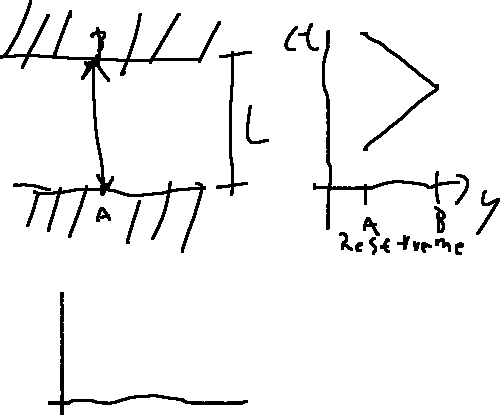
\includegraphics[width=10cm]{1-09-1.png}
	\caption*{Diagram of worldlines for the mirrors}
\end{figure*}
In an inertial frame if we consider two mirrors, then we see the round trip time will be $\Delta t = \frac{2L}{c}$. We can alos condsider this in a boosted frame, moving at a velocity $v$ in parallel to the surface of the mirrors, we see:
\begin{align*}
	\Delta x' &= v \Delta t' \\
	D &= 2\sqrt{L^2 + \left(\frac{\Delta x'}{2}\right)^2} \\
	\Delta t' &= \frac{2}{c}\sqrt{L^2 + \left(\frac{\Delta x'}{2}\right)^2}
\end{align*}

If we now consider the quantity $-(c\Delta t)^2 + (\delta \bm{r})^2$ in each coordinate system. In the boosted frame:
\begin{align*}
	-(c\Delta t')^2 + (\Delta x')^2 &= -4 (L^2 + \frac{\Delta x'\ ^2}{4}) + \Delta x'\ ^2 \\
	-(c\Delta t')^2 + (\Delta x')^2 &= -4 L^2 \\
	-(c\Delta t')^2 + (\Delta x')^2 &= -(c\Delta t)^2
\end{align*}
So it is the same in both frames.

This introduces the principle of relativity which say that our line element that defines distince have the same form in all inertial frames. In flat spacetime this line element is the one chosen above:
\begin{align*}
	ds^2 = -(c dt)^2 + dx^2 + dy^2 + dz^2
\end{align*}
Which we refer to as Minkowski space/the Minkowski line element.

From now on lowercase letters refer to spacetime, and uppercase letters refer to just space.

We say that particles with mass move along time-like world lines.

To measure distance along the worldline we'll use a ``proper time'' $\tau$ where $d\tau^2 = -\frac{ds^2}{c^2}$. We can say that two events are spacelike seperated if $(\Delta s)^2 >0$, timelike seperated if $(\Delta s)^2 <0$, and null for $(\Delta s)^2 =0$.

\subsection{Lorentz Boosts}
We will soon start dropping the factors of $c$ in many equations accepting the convention that $c=1$. 
In order to handle changing frames with a constant velocity between them, we need to use what's known as the Lorentz boost to transform instead of our simple Galilean boost.
This transformation will mix spatial and temporal dimensions in a manner somewhat analagous to rotations in Euclidean geometry:
\begin{align*}
	ct' &= \cosh\theta ct - \sinh\theta x \\
	x' &= -\sinh\theta ct + \cosh\theta x \\
	y' &= y \\
	z' &=z
\end{align*}
If we look at a worldline of a stationary particle in the boosted frame, we can see it corresponds to a constant velocity of $c\tanh\theta$ in the unboosted frame. Since $\cosh^2\theta -\sinh^2\theta = 1$ we can see:
\begin{align*}
	t' &= \gamma\left(t - \frac{vx}{c^2}\right) \\
	x' &= \gamma\left(x - v t\right) \\
	y' &= y \\
	z' &= z
\end{align*}
If we take the small velocity limit $v \ll c$, then:
\begin{align*}
	t' &= t \\
	x' &= x - v t \\
	y' &= y \\
	z' &= z
\end{align*}

We will now additionally add the conventions that we will use throughout the class. 
We will use the zeroeth index to refer to time throughtout the class, and will additionally use the einstein summation notation, i.e. $a^\alpha \hat{e}_\alpha = \sum_\alpha a^\alpha \hat{e}_\alpha$. 
We will also use greek indicies for all 4 spacetime coordinates, and latin indicies for only the spatial components.

The Lorentz boost of a vecotr is:
\begin{align*}
	a^t\ ' &= \gamma(a^t - va^x) \\
	a^x\ ' &= \gamma(a^x - va^t) \\
	a^y\ ' &= a^y \\
	a^z\ ' &= a^z
\end{align*}
And a scalar product is defined:
\begin{align*}
	\bm{a}\cdot\bm{b} &= (a^\alpha b^\beta) (\hat{e}_\alpha\cdot \hat{e}_\beta) \\
	\bm{a}\cdot\bm{b} &= (a^\alpha b^\beta) \eta_{\alpha\beta}
\end{align*}
Where for minkowski space:
\begin{align*}
	\eta_{\alpha\beta} &= \begin{pmatrix}
		-1 & 0 & 0 & 0 \\
		0 & 1 & 0 & 0 \\
		0 & 0 & 1 & 0 \\
		0 & 0 & 0 & 1
			      \end{pmatrix}
\end{align*}
So in flat space:
\begin{align*}
	\bm{a}\cdot\bm{b} &= -a^tb^t + a^x b^x + a^y b^y + a^z b^z
\end{align*}

When talking about worldilines we will typically refer to the position as a function of proper time, and a four velocity $u^\alpha = \frac{d x^\alpha}{d\tau}$. This can be written in terms of the three velocity:
\begin{align*}
	u^t &= \frac{dt}{d\tau} \\
	u^t &= \frac{1}{\sqrt{1-v^2}} \\
	u^i &= \frac{dx^i}{d\tau} \\
	u^i &= \frac{v^i}{\sqrt{1-v^2}} \\
	u^\alpha &= (\gamma,\gamma v^i)
\end{align*}

If we now compute the magnitude of $u^\alpha$, i.e. $u_\alpha u^\alpha = -1$

\subsection{Dynamics}
In the abscencce of outside forces, we should have constant 4 velocities, so (in any inertial frame):
\begin{align*}
	\frac{d u^\alpha}{d\tau} &= 0
\end{align*}
If we have a force applied though we see:
\begin{align*}
	m\frac{d u^\alpha}{d\tau} &= f^\alpha
\end{align*}
We say this is a 4 acceleration $a^\alpha = \frac{d u^\alpha}{d\tau}$, so we have $f^\alpha = m a^\alpha$.
We additionally say we have a 4 momentum $p^\alpha = m u^\alpha$, where clearly $p^\alpha p_\alpha = -m^2$.
If we look at our 4 momentum in terms of it's components in flat space:
\begin{align*}
	p^t &= \frac{m}{\sqrt{1-v^2}} \\
	p^i &= \frac{mv^i}{\sqrt{1-v^2}}
\end{align*}
In a low velocity limit we see:
\begin{align*}
	p^t &\approx m + \frac{m}{2}v^2 \\
	p^i &= m v^i
\end{align*}
So we can say (if we include a constant ress mass energy) $p^\alpha = (E,p^i)$


We know that in special relativity we must have our velocities sum in such a way that the velocity of light will not change, but the velocity of slower objects will (and in the non-relativistic limit they simply add).
We can say:
\begin{align*}
	dt' &= \gamma(dt - vdx) \\
	dx' &= \gamma(dx -v dt) \\
	\frac{dx'}{dt'} &= \frac{\frac{dx}{dt} - v}{1 -v \frac{dx}{dt}}
\end{align*}
If we choose $\frac{dx}{dt} = 1$ then $\frac{dx'}{dt'} = 1$. So this works for light like velocities how we want it to.

\subsection{Four vectors and coordinate systems}
We can write our line element in terms of our metric:
\begin{align*}
	ds^2 &= \eta_{\alpha\beta} dx^\alpha dx^\beta
\end{align*}
We tend to paramterize paths in terms of the proper time of the particle while moving. So our four velocity in terms of the proper time is then:
\begin{align*}
	u^\alpha &= \frac{dx^\alpha}{d\tau}
\end{align*}
Our temporal component is then going to be $u^t = \gamma$ and our spatial components are $u^i = \gamma v^i$, so we cam say our four velocity is then $u^\mu = (\gamma,\gamma \bm{V}$
\subsection{Dynamics}
We now consider Newton's first law in special relativity:
\begin{align*}
	\frac{d u^\mu}{d\tau} &= 0
\end{align*}
In the abscence of forces. In order to posit Newton's second law, we want it to abey this in the abscence of forces, be properly relativistic, and reduce to the classical result in the non-relativistic limit:
\begin{align*}
	m\frac{du^\mu}{d\tau} &= f^\mu
\end{align*}
Which since this is a 4-vector equation obviously obeys relativity, and it clearly obeys the first law when $f^\mu =0$. In order to check the classical limit, we define the four acceloration $a^\mu = \frac{du^\mu}{d\tau}$.
This gives us the classic $f^\mu = m a^\mu$. This is a set of 4 equations, which is one more than our classical set of equations. This is of course constrained by our restriction on the length of $u$, $u^\mu u_\mu = -1$, so:
\begin{align*}
	m \frac{d}{d\tau} u^\mu u_\mu &= 0 \\
	u^\mu a_\mu &= 0 \\
	f_\mu u^\mu &=0
\end{align*}
We now look at energy and momentum.
\begin{align*}
	p^\mu &= m u^\mu \\
	\frac{dp^\mu}{d\tau} &= f^\mu \\p^\mu p_\mu &= -m^2 \\
	p^t &= \frac{m}{1-v^2} \\
	p^i &= \frac{mv^i}{\sqrt{1-v^2}}
\end{align*}
If we take the limit where $v\ll 1$:
\begin{align*}
	p^t &= m + \frac{1}{2} mv^2 \\
	p^i &= mv^i
\end{align*}
So we say $p^\mu = (E, P)$

We now look to extract our spatial forces from our 4 force. We define this by $F^i = \frac{dP^i}{dt}$, so:
\begin{align*}
	f^i &= \frac{dP^i}{d\tau} \\
	f^i &= \gamma F^i
\end{align*}
We also know:
\begin{align*}
	f^t u^t &= f_i u^i \\
	f_t\gamma &= \gamma^2 F_i V^i \\
	f^t &= \gamma F_i V^i \\
	f^\mu &= (\gamma F_i V^i, \gamma F^i)
\end{align*}
\section{Curved Spacetime}
We say that our line element:
\begin{align*}
	ds^2 &= -dt^2 + dx^2 + dy^2 + dz^2
\end{align*}
Can be used to find line elements in other coordinate systems, such as with spherical coordinates. Here we will have:
\begin{align*}
	ds^2 &= -dt^2 + dr^2 + r^2 d\theta^2 + r^2\sin^2\theta d\phi^2
\end{align*}
This introduces a coordinate singularity, as if you choose $\theta=0$ all values for $\phi$ are mapped to the same point. This is non-physical though as it doesn't appear in caresian coordinates.

Let us now consider 2-D polar coordinates in flat space:
\begin{align*}
	dS^2 &= dr^2 = r^2d\phi^2
\end{align*}
If we transform to $r = \frac{a^2}{r'}$:
\begin{align*}
	dS^2 &= \frac{a^4}{r'\ ^4} (dr'\ ^2 + r'\ ^2 d\phi^2)
\end{align*}
Which has an infinite line element at $r' = 0$, but this makes sense as our transformation only gives us $r' = 0$ if $r = \infty$.
\subsection{Penrose diagrams}
We begin with our line element for flat spacetime in spherical coordinates:
\begin{align*}
	ds^2 &= -dt^2 + dr^2 + r^2 d\theta^2 + r^2\sin^2\theta d\phi^2
\end{align*}
We now define a coordinate $u = t - r$ and $v = t + r$, then we see we have a new line element:
\begin{align*}
	ds^2 &= -dudv + \frac{1}{4} (u-v)^2 (d\theta^2 \sin^2\theta d\phi^2)
\end{align*}
This implies off diagonal metric elements. In this coordinate system, lines of constant $u$ and $v$ are light paths.

We now make one more transformation:
\begin{align*}
	u' &= \arctan u &
	u' &= \frac{t' - r'}{2} \\
	v' &= \arctan{v} &
	v' &= \frac{t' + r'}{2}
\end{align*}
This will map all $(t,r)$ to $r' > 0$, $v' < \frac{\pi}{2}$, $u' > -\frac{\pi}{2}$
\begin{figure*}[h]
	\centering
	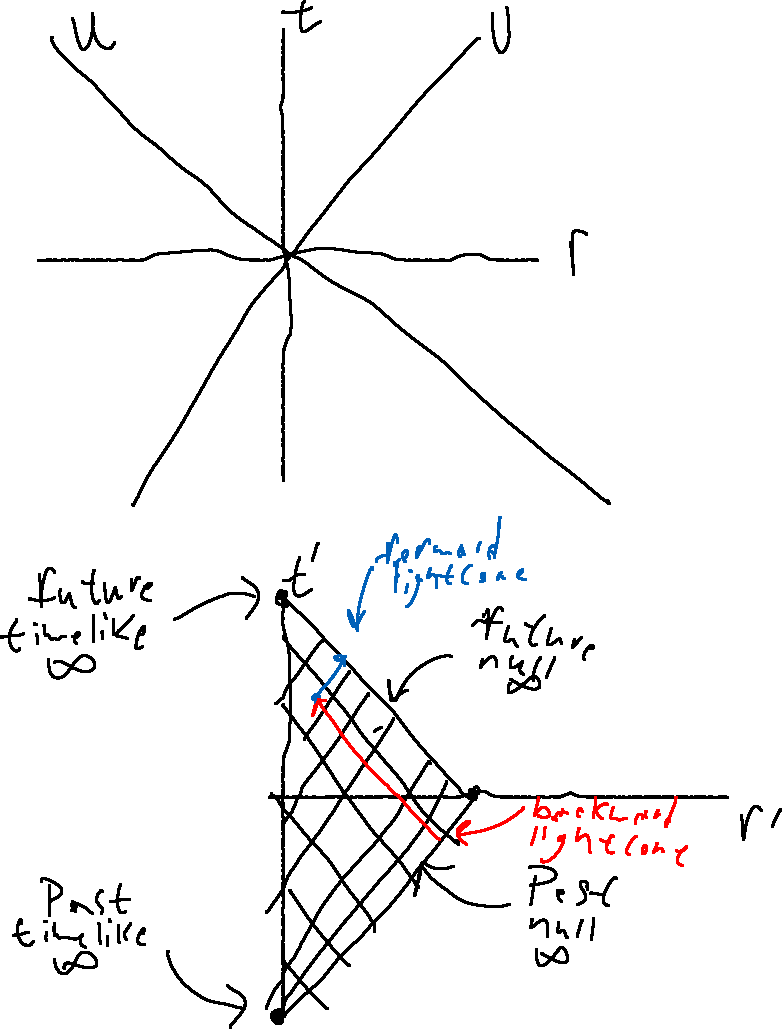
\includegraphics[width=6cm]{1-14-1.png}
	\caption*{Penrose Diagrams}
\end{figure*}
\subsection{Local Inertial frames}
We say that the equivalence priciple states that in local coordinates it is impossible to determine whether or not you are in curved spacetime.

In general we refer to our metric as $g_{\alpha\beta}$. Given some general metric (as a function of spacetime) $g_{\alpha\beta}(\bm{x})$, at every point $P$ we can invent a new coordinate system where:
\begin{align*}
	g_{\alpha\beta}'(x'_P) &= \eta_{\alpha\beta} \\
	\partder{g_{\alpha\beta}}{x'}|_P &= 0
\end{align*}
Which defines a local inertial frame at $p$.

Just as before we have the following types of distance:
\begin{align*}
	ds^2 < 0 & \text{timelike} \\
	ds^2 &= 0 & \text{null/lightlike} \\
	ds^2 >0 & \text{spacelike}
\end{align*}
Where our proper time can be defined as:
\begin{align*}
	\tau_{AB} &= \int_A^B \sqrt{-g_{\alpha\beta}(x)dx^\alpha dx^\beta}
\end{align*}
\subsection{Length, area, volume, and 4-volume}
For now we consider:
\begin{align*}
	ds^2 &= g_{00} (dx^0)^2 + g_{11}(dx^1)^2 + g_{22} (dx^2)^2 + g_33(dx^3)^2
\end{align*}
Therefore our area can be expressed as (for a rectangle in $x^1$, $x^2$):
\begin{align*}
	dA &= \sqrt{g_{11} g_{22}} dx^1 dx^2
\end{align*}
And for our three volume:
\begin{align*}
	dV &= \sqrt{g_{11}g_{22}g_{33}} dx^1 dx^2 dx^3 
\end{align*}
and finally four volume:
\begin{align*}
	dv &= \sqrt{-g_{00}g_{11}g_{22} g_{33}}dx^0dx^1dx^2dx^3
\end{align*}
If we let $g$ denote $\det g_{\alpha\beta}$ then:
\begin{align*}
	dv &= \sqrt{g} d^4 x
\end{align*}

We now consider the line element:
\begin{align*}
	dS^2 &= \frac{dr^2}{1-\left(\frac{r}{a}\right)^2} + r^2(d\theta^2 + \sin^2\theta d\phi^2)
\end{align*}
If we look at $r=R$ and $\theta = \frac{\pi}{2}$ then we calculate our circuference:
\begin{align*}
	C &= \oint dS \\
	C &= 2\pi R
\end{align*}
And then the distance from the center to the surface alone a line of constant $\theta$ and $\phi$:
\begin{align*}
	S &= \int dS \\
	S &= a\arcsin \frac{R}{a}
\end{align*}
Looking at the area of our surface at constant radius we find:
\begin{align*}
	A &= \int dA \\
	A &= 4\pi R^2
\end{align*}
And we finally consider the volume inside a radius $R$:
\begin{align*}
	V &= \int dV \\
	V &= \int_0^R dr\in_0^\pi d\theta\int_0^{2\pi}d\phi \frac{r^2\sin\theta}{1-\left(\frac{r}{a}\right)^2} \\
	V &= 4\pi a^3 \left(\frac{1}{2}\arcsin\left[\frac{R}{a}  - \frac{R}{2a} \sqrt{1 - \left(\frac{R}{a}\right)^2}\right]\right)
\end{align*}

\subsection{Embedding Diagrams}
We consider the line element:
\begin{align*}
	ds^2 &= -dt^2 + dr^2 +(b^2 + r^2)(d\theta^2 + \sin^2\theta d\phi^2)
\end{align*}
(Note we call this a static metric since there is no explicit time dependance). This is flat when $b=0$ but is not flat otherwise.

We now consider a slice where $t$ is constant:
\begin{align*}
	dS^2 &= dr^2 +(b^2 + r^2)(d\theta^2 + \sin^2\theta d\phi^2)
\end{align*}
And now constant angle ($\theta = \frac{\pi}{2}$:
\begin{align*}
	d\Sigma^2 &= dr^2 +(b^2 + r^2)d\phi^2
\end{align*}
We now consider this in cylindrical coordinates in flat space:
\begin{align*}
	dS^2 &= d\rho^2 + \rho^2 d\psi^2 + dz^2
\end{align*}
We look at this in terms of $z= z(r)$, $\rho = \rho(r)$ and $\psi = \phi$
We then have:
\begin{align*}
	d\psi &= d\phi \\
	dz &= \frac{dz}{dr} dr \\
	d\rho &= \frac{d\rho}{dr} dr
\end{align*}
So then:
\begin{align*}
	d\Sigma^2 &= \left(\frac{d\rho}{dr}\right)^2 dr^2 + \rho^2d\phi^2 + \left(\frac{dz}{dr}\right)^2 dr^2 \\
	d\Sigma^2 &= \left[\left(\frac{d\rho}{dr}+ \left(\frac{dz}{dr}\right)^2 \right)^2\right] dr^2 + \rho^2d\phi^2
\end{align*}
So then by inspection:
\begin{align*}
	\rho^2 &= r^2 + b^2 \\
	\left(\frac{dz}{dr}\right)^2 + \left(\frac{d\rho}{dr}\right)^2 &= 1 \\
	\left(\frac{d\rho}{dr}\right)^2 &= \frac{r^2}{\rho^2} \\
	\left(\frac{d\rho}{dr}\right)^2 &= \frac{r^2}{r^2 + b^2} \\
	\left(\frac{dz}{dr}\right)^2 &= \frac{1}{1 + \left(\frac{r}{b}\right)^2} \\
	z &= b\text{arcsinh}\frac{r}{b}
\end{align*}


Rewriting this in terms of $\rho$ we find:
\begin{align*}
	\sinh\frac{z}{b} &= \sqrt{\left(\frac{\rho}{b}\right)^2 - 1} \\
	\sinh^2\frac{z}{b} &= \left(\frac{\rho}{b}\right)^2 - 1 \\
	\frac{\rho}{b} &= \cosh \frac{z}{b}
\end{align*}
\begin{figure*}[h]
	\centering
	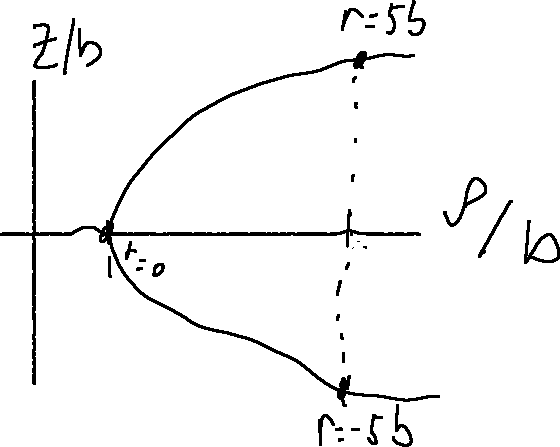
\includegraphics[width=6cm]{1-16-1.png}
	\caption*{Our embedding diagram}
\end{figure*}
Passing through $r=0$ here refers to moving to a distinct region of spacetime that is still flat but not the region of spacetime that we reached in the positive direction.
\subsection{Vectors in curved spacetime}
First we say that a vector is defined at a point in spacetime. Vector fields are generally functions of spacetime:
\begin{align*}
	\bm{a} &= \bm{a}(x^\mu)
\end{align*}
We now extend our basis vectors to be vector fields that are position dependant, i.e.:
\begin{align*}
	\bm{a} &= a^\alpha(x^\mu) \bm{e}_\alpha(x^\mu)
\end{align*}
So our dot product becomes:
\begin{align*}
	\bm{a}\cdot\bm{b} &= (\bm{e}_\alpha\cdot\bm{e}_\beta)a^\alpha b^\beta
\end{align*}
If we define a locally flat frame we conventionallly write: $\bm{e}_{\hat{\alpha}} \cdot\bm{e}_{\hat{\beta}} = \eta_{\hat{\alpha}\hat{\beta}}$.
These locally flat frames describe how an observer would view things. We do that by saying $\bm{e}_{\hat{t}} = \bm{u}_\text{obs}$.

Additionally we will have a coordinate basis where:
\begin{align*}
	u^\alpha &= \frac{dx^\alpha}{d\tau}
\end{align*}
Which in general will not be the same as our locally flat or orthonormal basis. We know that:
\begin{align*}
	\bm{u}\cdot\bm{u} &= -1 \\
	ds^2 &= g_{\alpha\beta}dx^\alpha dx^\beta \\
	ds^2 &= -d\tau^2
\end{align*}
We say we can write:
\begin{align*}
	g_{\alpha\beta}u^\alpha u^\beta &= -1
\end{align*}
In the coordinate basis.

To define the coordinate basis we say it is the basis in which:
\begin{align*}
	\bm{e}_\alpha(x^\mu)\cdot\bm{e}_\beta(x^\mu) &= g_{\alpha\beta}(x^\mu)
\end{align*}

So in summary we use our coordinate basis to do calculations, while we use orthonormal/locally flat basis to do interpretations. We will also use $\hat{\alpha}$ to refer to our orthonormal basis.

We now consider a coordinate basis and an orthonormal basis:
\begin{align*}
	\bm{a} &= a^\alpha\bm{e}_\alpha \\
	\bm{a} &= a^{\hat{\alpha}}\bm{e}_{\hat{\alpha}}
\end{align*}
In order to transform between these we need to express the components in terms of the other set of basis vectors, i.e:
\begin{align*}
	a^\alpha &= a^{\hat{\beta}}(\bm{e}_{\hat{\beta}})^\alpha \\
	a^{\hat{\alpha}} &= a^{\beta}(\bm{e}_{\beta})^{\hat{\alpha}}
\end{align*}
\subsection{Geodesics}
THe worldline of a free test particle between two timelike seperated points will exteremize the proper time between them. These extermized paths are known as geodesics, and the equations of motion that determine them are known as the geodesic equations.

For example we consider the equations for geodesics in plane in polar coordinates.
\begin{align*}
	dS^2 &= dr^2 + r^2 d\phi^2
\end{align*}
We describe a curve betwweeen two points $A$ and $B$ parametrically as $r(\sigma)$ and $\phi(\sigma)$, where $\sigma\in[0,1]$:
\begin{align*}
	S_{AB} &= \int_A^B dS \\
	S_{AB} &= \int_0^1 d\sigma \sqrt{\left(\frac{dr}{d\sigma}\right)^2 + r^2 \left(\frac{d\phi}{d\sigma}\right)^2}
\end{align*}
We can see that this defines a lagrangian:
\begin{align*}
	\mathcal{L}&= \sqrt{\left(\frac{dr}{d\sigma}\right)^2 + r^2 \left(\frac{d\phi}{d\sigma}\right)^2} \\
	\frac{d}{d\sigma} \left(\frac{1}{\mathcal{L}} \frac{dr}{d\sigma}\right) &= \frac{r}{\mathcal{L}} \left(\frac{d\phi}{d\sigma}\right)^2 \\
	\frac{d^2r}{ds^2} &= r\left(\frac{d\phi}{ds}\right)^2
\end{align*}

The equations for time-lke geodesics will be talked about in terms of proper time:
\begin{align*}
	\tau_{AB} &= \int_A^Bd\tau \\
	\tau_{AB} &= \int_A^B\sqrt{-g_{\alpha\beta}(x) dx^\alpha dx^\beta} \\
	\tau_{AB} &= \int_0^1d\sigma\sqrt{-g_{\alpha\beta}(x) \frac{dx^\alpha}{d\sigma} \frac{dx^\beta}{d\sigma}}
\end{align*}
Which gives us a Lagrangian:
\begin{align*}
	\mathcal{L} &= \sqrt{-g_{\alpha\beta}(x)\frac{dx^\alpha}{d\sigma}\frac{dx^\beta}{d\sigma}}
\end{align*}
Where:
\begin{align*}
	\partder{\mathcal{L}}{dx^\alpha} &= \frac{d}{d\sigma} \partder{\mathcal{L}}{\frac{dx^\alpha}{d\sigma}}
\end{align*}

We now return to our wormhole geometry:
\begin{align*}
	ds^2 &= -dt^2 + dr^2 + (r^2 + b^2)(d\theta^2 + \sin^2\theta d\phi^2) \\
	\mathcal{L} &= \sqrt{\left(\frac{dt}{d\sigma}\right)^2 - \left(\frac{dr}{d\sigma}\right)^2 0 (b^2 + r^2)\left[\left(\frac{d\theta}{d\sigma}\right)^2 + \sin^2\theta \left(\frac{d\phi}{d\sigma}\right)^2\right]}
\end{align*}
We note that $\partder{\mathcal{L}}{()} \propto \frac{1}{\mathcal{L}}$ and we also see:
\begin{align*}
	\mathcal{L} &= \frac{d\tau}{d\sigma} \\
	\partder{\mathcal{L}}{t} &= 9 &
	\frac{d^2 t}{d\tau^2} &= 0 \\
	\partder{\mathcal{L}}{r} &= -\mathcal{L}r\left[\left(\frac{d\theta}{d\sigma}\right)^2 + \sin^2\theta \left(\frac{d\phi}{d\sigma}\right)^2\right] \\
	\partder{\mathcal{L}}{\frac{dr}{d\sigma}} &= -\frac{d r}{d\tau}
\end{align*}
WHich then implies:
\begin{align*}
	\frac{d^2 r}{d\tau^2} &= r\left[\left(\frac{d\theta}{d\sigma}\right)^2 + \sin^2\theta \left(\frac{d\phi}{d\sigma}\right)^2\right] \\
\end{align*}
We now look at the rest of the problem:
\begin{align*}
	\frac{d}{d\tau} \left[(b^2 + r^2)\frac{d\theta}{d\tau}\right] &= (b^2 + r^2)\sin\theta\cos\theta\left(\frac{d\theta}{d\tau}\right)^2 \\
	\frac{d}{d\tau} \left[(b^2+ r^2)\sin^2\theta \frac{d\phi}{d\tau}\right] &= 0
\end{align*}

The general form of the geodesic equation for timelike geodesics will be:
\begin{align*}
	\frac{d^2x^\alpha}{d\tau^2} &= -\Gamma_{\beta\gamma}^\alpha \frac{dx^\beta}{d\tau} \frac{dx^\gamma}{d\tau}
\end{align*}
This is a set of for equations, one for each $\alpha$. The $\Gamma$ symbols are called the Christoffel symbols, are constructed from our metric and 1st derivitives, and are notably not tensors:
\begin{align*}
	u^z\alpha &= \frac{dx^\alpha}{d\tau} \\
	\frac{du^\alpha}{d\tau} &= -\Gamma_{\beta\gamma}^\alpha u^\beta u^\gamma
\end{align*}
These are symmetric in the lower indicies.
`
Looking back at the plane in polar coordinates:
\begin{align*}
	\frac{d^2 r}{dS^2} &= r \left(\frac{d\phi}{dS}\right)^2 &
	\frac{d}{dS} \left(r^2 \frac{d\phi}{dS} \right) &= 0 \\
	\Gamma_{\phi\phi}^r &= -r &
	\Gamma_{r\phi}^\phi &= \frac{1}{r}
\end{align*}
Where all the others will be 0.

We can additionally compute the Chrisoffel symbols via:
\begin{align*}
	g_{\alpha\delta}\Gamma_{\beta\gamma}^\delta &= \frac{1}{2}\left(\partder{g_{\alpha\beta}}{x^\gamma} + \partder{g_{\alpha\gamma}}{x^\beta} - \partder{g_{\beta\gamma}}{x^\alpha}\right)
\end{align*}


We now look to compute the travel time through a wormhole geometry as an example. We have our traveler begin at a coordinate radius $R$ and allow them to fall inward through the Wormhole.
Therefore we say:
\begin{align*}
	u^r &= U
\end{align*}
So we have an initial radial 4-velocity. We now attempt to compute the time the traveler experiences traveling to $r=-R$. In order to have the total length of our 4-velocity equal to $-1$ we say:
\begin{align*}
	\bm{u} &= (\sqrt{1+ U^2},U,0,0)
\end{align*}
We can see from our prior work in this geometry:
\begin{align*}
	\partder{u^r}{\tau} &= 0
\end{align*}
So moving along the radius we see that the radial component is constant and therefore we can say:
\begin{align*}
	r(\tau) &= U\tau \\
	\Delta\tau &= \frac{2R}{U}
\end{align*}
Recall from mechanics, that conservation laws give first integrals of EOM, which generally reduce the number of equations we need to solve.
In GR we know that the four velocity's length is always conserved $g_{\alpha\beta} u^\alpha u^\beta = -1$.
Symmetries in our spacetime will give us other conservation laws. From Newtonian mechanics we know that energy conservation arises from a potential that is invariant under time translation.
Conserved linear momentum arrises from translation invariance. For angular momentum we see a conservation law will arise from rotational invariance (spherical symmetry).

In GR we look at symmetries in spacetime. These occur when the metric is invariant under displacements in a given coordinate.
The four vector $\xi = (0,1,0,0)$ which captures our symmetry is called the Killing vector associated with the symmetry.

For example in flat space:
\begin{align*}
	dS^2 &= dx^2 + dy^2 + dz^2
\end{align*}
We can immediately see that we have killing vectors $(1,0,0)$, $(0,1,0)$, and $(0,0,1)$. We can see if we change coordinate to spherical coordinates we have:
\begin{align*}
	dS^2 &= dr^2 + r^2 d\theta^2 + r^2\sin^2\theta d\phi^2
\end{align*}
So we can see we have the killing vector $(0,0,1)$.

These killing vectors are associated with constants of motion: 
\begin{align*}
	\bm{\xi}\cdot\bm{u} &= \text{const}
\end{align*}
If our metric (and therefore our Lagrangian) are independant of some coordinate $x^1$, then:
\begin{align*}
	\partder{\mathcal{L}}{x^1} &=0 \\
	\frac{d}{d\sigma} \partder{\mathcal{L}}{\frac{dx^1}{d\sigma}} &= 0 \\
	\partder{\mathcal{L}}{\frac{dx^1}{d\sigma}} &= -g_{1\beta} \frac{1}{\mathcal{L}} \frac{dx^\beta}{d\sigma} \\
	\partder{\mathcal{L}}{\frac{dx^1}{d\sigma}} &= -g_{1\beta} \frac{dx^\beta}{d\tau} \\
	\partder{\mathcal{L}}{\frac{dx^1}{d\sigma}} &= -g_{\alpha\beta} \xi^\alpha\frac{dx^\beta}{d\tau} \\
	\partder{\mathcal{L}}{\frac{dx^1}{d\sigma}} &= -\bm{\xi}\cdot\bm{u}
\end{align*}
Looking now at null geodesics (the paths of photons). We can no longer use proper time to parameterize our paths since photons have $\Delta\tau = 0$. We choose our parameter to be $\lambda$, so:
\begin{align*}
	u^\alpha &= \frac{dx^\alpha}{d\lambda} \\
	\bm{u}\cdot\bm{u} &= g_{\alpha\beta} \frac{dx^\alpha}{d\lambda} \frac{dx^\beta}{d\lambda} \\
	\bm{u}\cdot\bm{u} &= 0
\end{align*}
We know in flat spacetime that:
\begin{align*}
	\frac{d^2x^\alpha}{d\lambda^2} &= 0
\end{align*}
We want to generalize this, and we want to be sure to maintain that: 1. in a local inertial frame our generalization reduces to this, and 2. that this takes the same form in all coordinate systems.

We choose as our generalization:
\begin{align*}
	\frac{d^2x^\alpha}{d\lambda^2} &= -\Gamma^\alpha_{\beta\gamma} \frac{dx^\beta}{d\lambda}\frac{dx^\gamma}{d\lambda}
\end{align*}

\subsection{Shwarzchild geometry}
We consider the geometry outside a spherical star:
\begin{align*}
	ds^2 &= -\left(1 -\frac{2GM}{c^2 r}\right)(cdt)^2 + \left(1- \frac{2GM}{c^2 r}\right)dr^2 + r^2 (d\theta^2 + \sin^2\theta d\phi^2)
\end{align*}
We refer to these coordinates as Schwarzchild coordinates. We can immediately see this is spherically symmetric, and that as $r\to\infty$ this becomes flat spacetime.
Additionally we see there are coordinate singularities at $r=0$ and $r=\frac{2GM}{c^2}$. The singularity at $r=0$ can be ignored for physical reasons, and the other one is because of the choice of coordinates, and can be removed by changing coordinates.
Also note that $r$ is not radial distance, but instead related to the surface area of a sphere of that radius. Also this is time independant. We can write killing vector:
\begin{align*}
	\xi &= (1,0,0,0)
\end{align*}
And the geometry at constant $r$ and $t$:
\begin{align*}
	d\Sigma^2 &= r^2(d\theta^2 + \sin^2\theta d\phi^2)
\end{align*}
Where we find another killing vector:
\begin{align*}
	\eta &= (0,0,0,1)
\end{align*}
We may assume that $M$ is the mass of the star, but we now want to interogate this by taking the non-relativistic limit:
\begin{align*}
	\frac{GM}{c^2 r} \ll 1 \\
	ds^2 &\approx -\left(1 - \frac{2GM}{c^2r}\right)(cdt)^2 + \left(1+ \frac{2GM}{c^2 r}\right)dr^2 + r^2 (d\theta^2 + \sin^2\theta d\phi^2)
\end{align*}
Which is the static weak field metric for the Newtonian gravitational potential

Looking at the Schwarzchild radius $r = \frac{2GM}{c^2}$.

Now we look at the effect on light of killing vectors moving away from the singularity of a shwarzchild geometry.
If we have an emission event at fixed radius R emitting a light signal with frequency $\omega_*$ and an infinitely distant observer sees it with frequence $\omega_\infty$.
We know the energy of this photon is $E=\hbar\omega$. And we have a symmetry related to this:
\begin{align*}
	\xi &= (1,0,0,0) \\
	\bm{\xi}\cdot\bm{p} &= \text{const}
\end{align*}
We want to move to orthonormal basis for our observers, in these frames we will have each observers velocity vector be $u = (1,0,0,0)$.

Therefore we say an observer moving with velocity $\bm{u}_\text{obs}$ will measure an energy:
\begin{align*}
	E &= -\bm{p}\cdot\bm{u}_\text{obs} \\
	E &= \hbar\omega
\end{align*}
For any observer we will have four velocity:
\begin{align*}
	\bm{u}_\text{obs}\cdot\bm{u}_\text{obs} &= -1
\end{align*}
In the observers frame:
\begin{align*}
	u_\text{obs}^i &= 0 \\
	g_{tt}(r) u^t_\text{obs}\ ^2 &= -1 \\
	u^t_\text{obs} &= \left(1- \frac{2GM}{c^2 r}\right)^{-\frac{1}{2}}
\end{align*}
So for our stationary observer:
\begin{align*}
	\bm{u}_\text{obs} &= \left(1- \frac{2GM}{c^2 r}\right)^{-\frac{1}{2}}\bm{\xi}
\end{align*}
So:
\begin{align*}
	\hbar\omega_* &= \left(1- \frac{2GM}{c^2 r}\right)^{-\frac{1}{2}}(\bm{\xi}\cdot\bm{p})_R \\
	\hbar\omega_\infty &= (\bm{\xi}\cdot\bm{p})_\infty
\end{align*}
But this is a conserved quantity, so:
\begin{align*}
	(\bm{\xi}\cdot\bm{p})_R &= (\bm{\xi}\cdot\bm{p})_\infty \\
	\omega_\infty &= \omega_* \sqrt{1 - \frac{2GM}{c^2 R}}
\end{align*}


We now look at particle motion in the Schwazchild geometry. We say that the metric will be independant of $t$ and $\phi$. I.e. we have constants:
\begin{align*}
	\bm{\xi}\cdot\bm{u} &= \text{const} &
	\xi &= (1,0,0,0) \\
	\bm{\eta}\cdot\bm{u} &= \text{const} &
	\eta &= (0,0,0,1)
\end{align*}
We say:
\begin{align*}
	e &= -\bm{\xi}\cdot\bm{u} \\
	e &= \left(1- \frac{2M}{r}\right) \frac{dt}{d\tau}
\end{align*}
Which is our conserved energy per unit mass. And we also have:
\begin{align*}
	l &= \bm{\eta}\cdot\bm{u} \\
	l &= r^2\
	sin^2\theta \frac{d\phi}{d\tau}
\end{align*}
Which is our conserved angular momentum per unit mass.

Since the four velocity must be normalized we can say:
\begin{align*}
	\bm{u}\cdot\bm{u} &= -1 \\
	\bm{u}\cdot\bm{u} &= g_{\alpha\beta} u^\alpha u^\beta \\
	\bm{u}\cdot\bm{u} &= -\left(1 - \frac{2M}{r}\right)(u^t)^2 + \left(1 - \frac{2M}{r}\right)^{-1}(u^r)^2 + r^2(u^\phi)^2
\end{align*}
Where we have picked coordinates where we are rotating in the plane $\theta = \frac{\pi}{2}$. Inserting our known constants of motion:
\begin{align*}
	\bm{u}\cdot\bm{u} &= -\left(1 - \frac{2M}{r}\right)e^2 + \left(1 - \frac{2M}{r}\right)^{-1}\left(\frac{dr}{d\tau}\right)^2 + \frac{l^2}{r^2}\\
	\frac{e^2 - 1}{2} &= \frac{1}{2}\left(\frac{dr}{d\tau}\right)^2 + \frac{1}{2}\left[\left(1-\frac{2M}{r}\right)\left(1+ \frac{l^2}{r^2}\right) - 1\right] \\
	\varepsilon &= \frac{e^2 - 1}{2} \\
	\varepsilon &= \frac{1}{2}\left(\frac{dr}{d\tau}\right)^2 + \frac{1}{2}\left[\left(1-\frac{2M}{r}\right)\left(1+ \frac{l^2}{r^2}\right) - 1\right]
\end{align*}
We then define an effective potential:
\begin{align*}
	V_\text{eff} &= \frac{1}{2}\left[\left(1-\frac{2M}{r}\right)\left(1+ \frac{l^2}{r^2}\right) - 1\right] \\
	V_\text{eff} &= -\frac{M}{r} + \frac{l^2}{2r^2} - \frac{Ml^2}{r^3} \\
	\varepsilon &= \frac{1}{2}\left(\frac{dr}{d\tau}\right)^2 + V_\text{eff}(r)
\end{align*}


\end{document}
